\chapter{Privacy}
\label{ch:privacy}


\only<article>{ What do we mean by privacy? One interpretation is
  simply the ability to maintain a personal secret. Is it possible to
  maintain perfect secrecy? Can the thoughts in our head be perfectly
  safe, or can they be revealed indirectly through our actions? 

  THe problems we will discuss in this chapter are \emph{not}
  solveable through cryptography. We certainly /emph{can} securely
  store and transmit data using cryptography. Through homomorphic
  computation, an untrusted server can even perform some computations
  on encrypted data, returning an encrypted result to us, while
  learning nothing about the original secret.  As long as the data, as
  well as any derivative information, using it is kept under lock and
  key, our personal information cannot be revealed.

  However, sometimes we must make public decisions or release public
  information based on this data. Then the data can be revealed
  indirectly. For example, you can trust your doctor to maintain
  confidentiality, but when you go to the pharmacy to get the
  prescribed medicine, somebody can infer the medical condition you
  suffer from.

  It is even possible to learn personal information from aggregate
  statistics.  Let us say your doctor publishes a list of cases of
  different diseases every week, together with some other information
  such as the approximate patient age. Even though your own data is
  mixed with that of all other patients, it is not difficult for
  somebody to infer your diagnosis, especially if they already have
  some additional side-information.

 
  We will emphasize an algorithmic view of privacy. Here, participants
  entrusts their data to an algorithm, which is in turn supposed to
  produce something useful in return. The algorithm is typically not
  fully automated, as it also depends on some human input. One example
  is a medical study examining different treatments for a
  disease. While humans select and administer the treatments, they
  will typically rely on a randomised strategy for assigning
  treatments to individuals, and use a statistical method to report
  their results. A navigation application would collect data from
  multiple users in real-time to be able to plan new routes and detect
  traffic jams. Given this mixture of ad-hoc decisions and formal
  algorithmic methods, is it possible to guarantee privacy in any
  sense? What kind of guarantees can we make?

  Generally speaking, an algorithm has good privacy properties, if the
  amount of information that can be revealed through the algorithm's
  output abound any individual contributing data is bounded. In
  particular, we are interested in how much an adversary can learn
  about the algorithm's input from the algorithm's output. This does
  not preclude learning general facts about individuals from the
  output. For example, a study about the use of steroids in sports may
  show that 90\% of sprinters with times under 10 seconds are using
  steroids. Any sprinter with a time under 10 seconds is thus tainted
  by association, even if their data has not been used in the
  study. The publication of the result, then, does not impact their
  privacy, even though it has a negative effect.
  
 
  
  In this chapter, we will look at two formal concepts of privacy
  protection: $k$-anonymity and \emph{differential privacy}. The first
  is a simple method for anonymising databases. However, it provides
  only limited resistance to identification. The latter is a more
  general concept, which provides full information-theoretic
  protection to individuals. A major problem with any privacy
  definition and method, however is correct interpretation of the
  privacy concept used, and correct implementation of the algorithm
  used.  }

\begin{frame}
  \centering
  \includegraphics[height=\textheight]{../figures/smbc-the-problem}
\end{frame}
\begin{frame}
  \only<article>{ ``Data is everywhere'', said the statistician,
    ``data, data!''. In the past, statistical analysis was performed
    with laboriously collected and annotated datasets. Even as
    recently as in the early 21st century, databases for machine
    learning were limited to a few thousand entries at most. At the
    time of writing, not only has the size of datasets become
    extremely large, but the sources of data are much more
    diverse. Data are collected and commercialised whenever we visit a
    website and even as we walk around with our phone. To a limited
    extent, there is a tradeoff between what we can get out of a
    service and what we pay into it. Many free services such as
    navigation software rely on collecting user data to perform
    better: If you can tell that there is a traffic jam in Central
    Avenue, you can after all try and take another route.  As long as
    informed consent exists, use of private data is generally regarded
    as unproblematic.\footnote{This is actually underscored by the
      GDPR legislation, which focuses on consent and data use
      methods.}

    However, even apparently benign data collected with appropriate
    consent can lead to serious and unexpected privacy
    violations. There are three famous examples of this: Firstly, the
    identification of people in supposedly anonymous health data in
    the 1990s in the state of Massachussets, which we will go over in
    detail in this chapter. Secondly, the identifications of users
    through anonymised movie ratings in the Netflix dataset. Finally,
    the ability to discover if any given individual's data is
    contained in a pooled genomic study.

    In this chapter, we will introduce one of the main tools for
    giving formal guarantees about the privacy of any algorithm ran on
    a dataset, \emph{differential privacy}. This will provide
    individual-level privacy, in the sense that an algorithm that is
    differentially private guarantees that no adversary can
    significantly increase their knowledge about any particular
    individual by observing the algorithm's output. This is independent
    of the adversary's existing knowledge, or computational power.
  }
  \begin{block}{Privacy in statistical disclosure.}
    \only<article>{ Consider a researcher wishing to collect data for a  statistical analysis. As long as the analysis is eventually
      published,\footnote{If somebody knows that the analysis is being
        conducted, however, they could still learn something private from the fact that the analysis has /emph{not} been published.} this
      creates two types of possible privacy violations.}
    \begin{itemize}
    \item Public analysis of sensitive data.
    \item Publication of ``anonymised'' data.
    \end{itemize}
    \only<article>{ The first is direct exposure of sensitive data
      through publication of the analysis, if for example the study is
      about something such as drug use. The second is through
      publication of ``anonymised'' versions of the dataset, for
      example by removing names and addresses, which create
      opportunities for linkage attacks.}
  \end{block}
  \begin{alertblock}{Not about cryptography}
    \only<article>{
      The problems we are considering can not be solved through cryptographic means. Cryptography provides:}
    \begin{itemize}
    \item Secure communication and computation.
    \item Authentication and verification.
    \end{itemize}
    \only<article>{These are useful to establish secure channels with somebody that we trust. However, the issue that}
  \end{alertblock}

  \begin{block}{An issue of trust}
    \only<article>{Fundamentally, privacy in statistics is an issue of trust. The analyst, whether it be a human statistician, or an automated service provided by a company, will use your data to make decisions. You must also decide:}
    \begin{itemize}
    \item Who to trust and how much.
    \item With what data to trust them.
    \item What you want out of the service.
    \end{itemize}
    \only<article>{These are difficult questions and are hard to quantify, hence in this course we are assuming that we have already decided how to answer them, and we simply want to find an appropriate methodology for achieving a good result.}
  \end{block}
\end{frame}


\section{Privacy in databases}
\only<presentation>{
  \begin{frame}
    \tableofcontents[ 
    currentsection, 
    hideothersubsections, 
    sectionstyle=show/shaded
    ] 
  \end{frame}
}

\only<article>{
  Every day ,
  
}
\begin{frame}
  \frametitle{Anonymisation}
  \only<article>{If we wish to publish a database, frequently we need to protect identities of people involved. The simplest method for doing that is simply erasing directly identifying information. However, this does not really work most of the time, especially since attackers can have side-information that can reveal the identities of individuals in the original data.
    
    
  }
  
  \begin{example}[Typical relational database in Tinder]
    \begin{table}[H]
      \begin{tabular}{l|l|l|l|l|l|l}
        Birthday & Name & Height  & Weight & Age & Postcode & Profession\\
        \hline
        06/07 & \only<1>{Li Pu} & 190 & 80 & 60-70 & 1001 & Politician\\
        06/14 & \only<1>{Sara Lee} & 185 & 110 & 70+ & 1001 & Rentier\\
        01/01 & \only<1>{A. B. Student} & 170 & 70 & 40-60 & 6732 & Time Traveller
      \end{tabular} 
    \end{table}
  \end{example}

  \only<2>{The simple act of hiding or using random identifiers is called anonymisation.}
  \only<article>{However this is generally insufficient as other identifying information may be used to re-identify individuals in the data.}
\end{frame}


\begin{frame}
  \frametitle{Record linkage}
  \begin{columns}
    \begin{column}{0.7\textwidth}
      \centering \def\firstcircle{(0,0) circle (7em)}
      \def\secondcircle{(3,0) circle (7em)}
      
      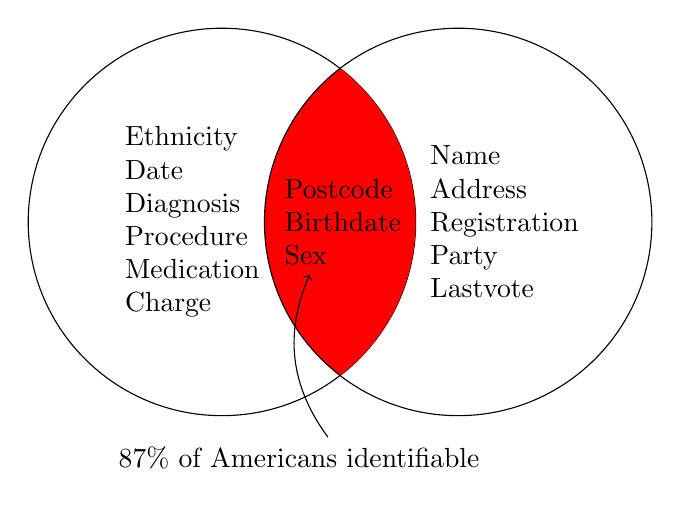
\begin{tikzpicture}
        \uncover<1,3>{ \draw \firstcircle node[text width=7em]
          {Ethnicity\newline Date\newline Diagnosis \newline Procedure
            \newline Medication \newline Charge }; } \uncover<3>{
          \begin{scope}
            \clip \firstcircle; \fill[red] \secondcircle;
          \end{scope}
        } \uncover<2,3>{\draw \secondcircle node [text width=2em,
          align=right] {Name \newline Address \newline Registration
            \newline Party \newline Lastvote}; } \node [text width=4em]
        (QI) at (1.5, 0) {Postcode \newline Birthdate \newline Sex};
        \uncover<3>{ \node [text width=16em] (qi-text) at (1.5, -3)
          {87\% of Americans identifiable}; \path[->]<1-> (qi-text) edge [bend left]
          (QI); }
      \end{tikzpicture}
    \end{column}
    \begin{column}{0.3\textwidth}
      \includegraphics[width=0.5\columnwidth]{../figures/Bill_Weld}
      \\
      Bill Weld, R-MA
    \end{column}
  \end{columns}
  \note{As an example, in the 1990s a study published anonymised information about the health records of individuals. They were careful to hide all obviously identifying information such as their name. However, a publically available database of voting records allowed attackers to cross-reference this data, and so obtain the identities of individuals in that database. Clearly, anonymisation is not enough. So, is there a way to formally guarantee privacy?}
\end{frame}
\begin{frame}
  \begin{example}[Typical relational database in a tax office]
    \begin{table}[H]
      \begin{tabular}{l|l|l|l|l|l|l}
        ID & Name &  Salary & Deposits & Age & Postcode & Profession\\
        \hline
        1959060783 & Li Pu & 150,000 & 1e6 & 60 & 1001 & Politician\\
        1946061408 & Sara Lee & 300,000 & -1e9 & 72 & 1001 & Rentier\\
        2100010101 & A. B. Student & 10,000 & 100,000 & 40 & 6732 & Time Traveller
      \end{tabular}
    \end{table}
  \end{example}
  
  \begin{example}[Typical relational database in a tax office]
    \begin{table}[H]
      \begin{tabular}{l|l|l|l|l|l|l}
        Birthday & Name & Height  & Weight & Age & Postcode & Profession\\
        \hline
        06/07 & & 190 & 80 & 60-70 & 1001 & Politician\\
        06/14 &  & 185 & 110 & 70+ & 1001 & Rentier\\
        01/01 &  & 170 & 70 & 40-60 & 6732 & Time Traveller
      \end{tabular}
    \end{table}
  \end{example}
\end{frame}

% \begin{frame}
%   \frametitle{Data linkage with SQL}
%   The original database \verb|database| and adversary side information \verb|side-information| can be combined using the following simple SQL query:
% \begin{verbatim}
% SELECT * FROM database JOIN side-information ON [condition]
% \end{verbatim}
%   where \verb|condition| describes how to match the records.

%   \begin{example}
%     For the databases given above, we could use
% \begin{verbatim}
% SELECT * FROM tinder JOIN tax ON tinder.height = tax.height AND tinder.age = tax.age
% \end{verbatim}
%     to create a joint table.
%   \end{example}
% \end{frame}

\section{$k$-anonymity}

\begin{frame}
  \frametitle{$k$-anonymity}
  \begin{figure}[H]
    \centering
    \begin{subfigure}{0.45\textwidth}
      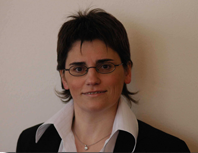
\includegraphics[width=0.25\textwidth]{../figures/samarati}
      \caption{Samarati}
    \end{subfigure}
    \begin{subfigure}{0.45\textwidth}
      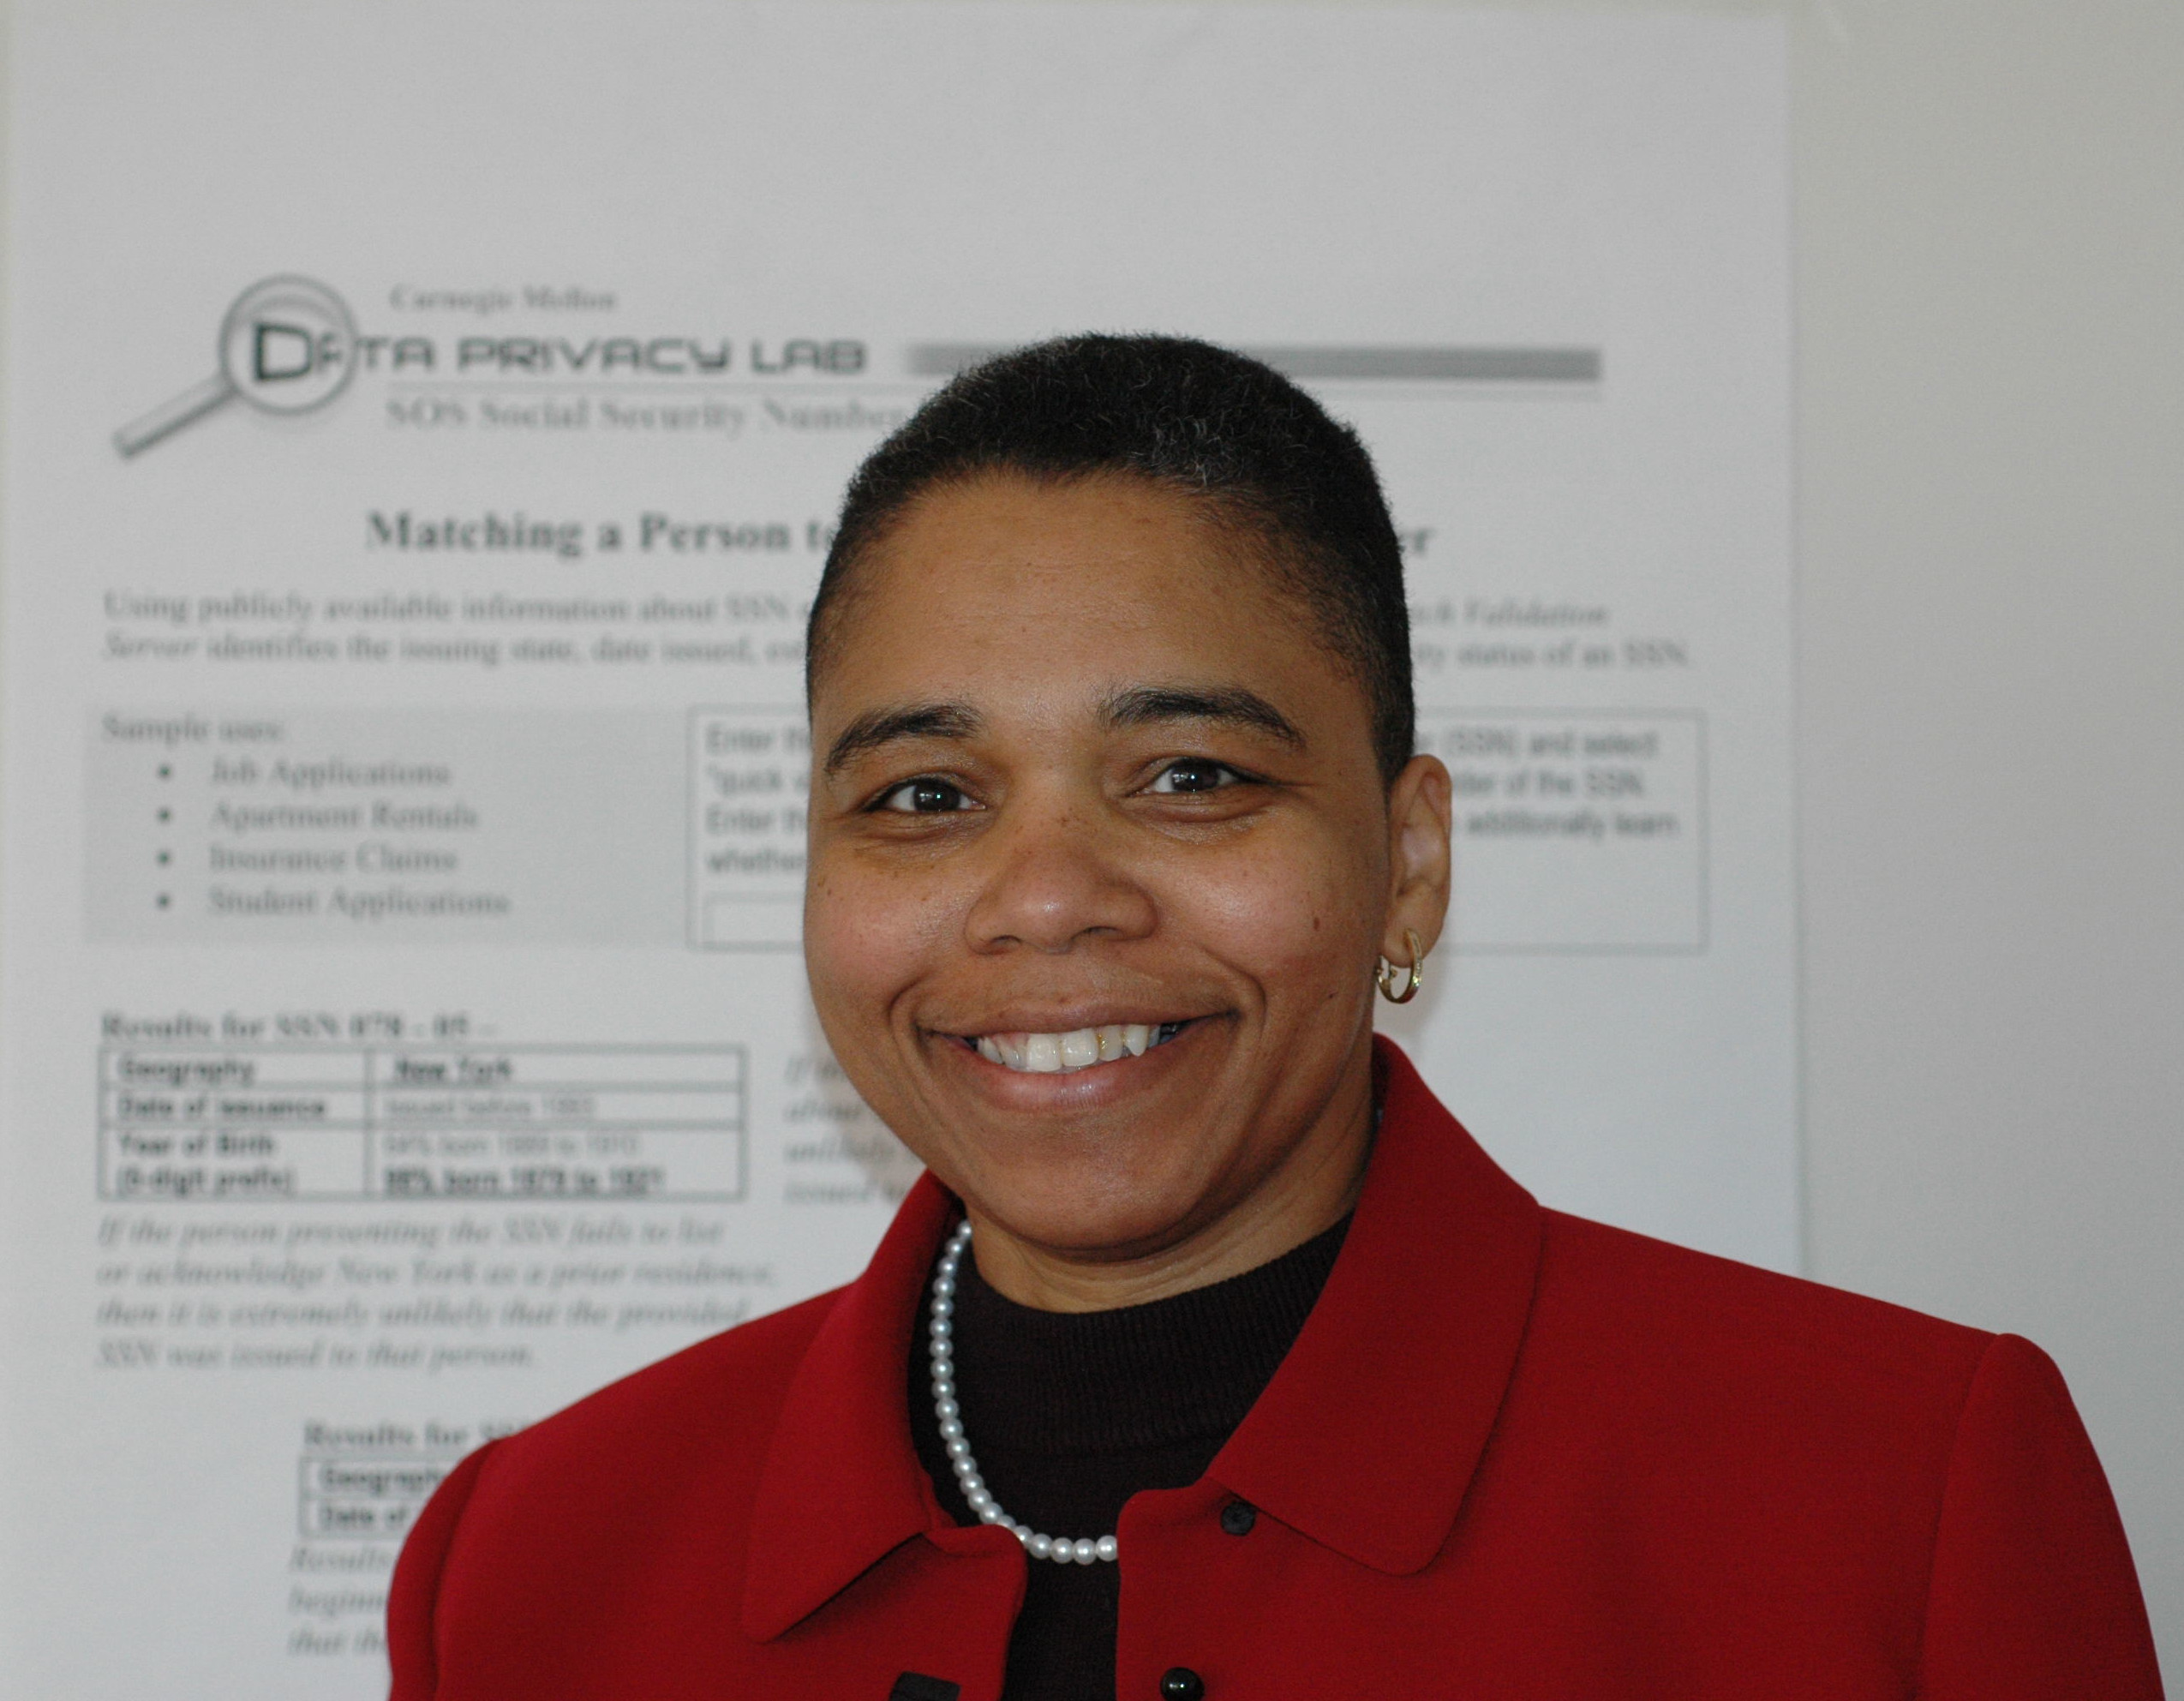
\includegraphics[width=0.25\textwidth]{../figures/sweeney}
      \caption{Sweeney}
    \end{subfigure}
  \end{figure}
  \only<article>{The concept of $k$-anonymity was introduced by~\citet{samarati1998protecting} and provides good guarantees when accessing a single database}

  \begin{definition}[$k$-anonymity]
    A database provides $k$-anonymity if for every person in the database is indistinguishable from $k-1$ persons with respect to \emph{quasi-identifiers}.
  \end{definition}
  \alert{It's the analyst's job to define quasi-identifiers}
  
\end{frame}

\begin{frame}
  \only<1>{
    \begin{table}[H]
      \begin{tabular}{l|l|l|l|l|l|l}
        Birthday & Name & Height  & Weight & Age & Postcode & Profession\\
        \hline
        06/07 & Li Pu & 190 & 80 & 60+ & 1001 & Politician\\
        06/14 & Sara Lee & 185 & 110 & 60+ & 1001 & Rentier\\
        06/12 & Nikos Papadopoulos & 180 & 82 & 60+ & 1243 & Politician\\
        01/01 & A. B. Student & 170 & 70 & 40-60 & 6732 & Time Traveller\\
        05/08 & Li Yang & 175 & 72 & 30-40 & 6910 & Time Traveller
      \end{tabular}
      \caption{1-anonymity.}
    \end{table}

  }
  \only<presentation>{
    \only<2>{
      \begin{tabular}{l|l|l|l|l|l|l}
        Birthday & Name & Height  & Weight & Age & Postcode & Profession\\
        \hline
        06/07 &  & 190 & 80 & 60+ & 1001 & Politician\\
        06/14 &  & 185 & 110 & 60+ & 1001 & Rentier\\
        06/12 &  & 180 & 82 & 60+ & 1243 & Politician\\
        01/01 &  & 170 & 70 & 40-60 & 6732 & Time Traveller\\
        05/08 &  & 175 & 72 & 30-40 & 6910 & Policeman
      \end{tabular}
      1-anonymity
    }

    \only<3>{
      \begin{tabular}{l|l|l|l|l|l|l}
        Birthday & Name & Height  & Weight & Age & Postcode & Profession\\
        \hline
        06/07 &  & 180-190 & 80+ & 60+ & 1* & \\
        06/14 &  & 180-190 & 80+ & 60+ & 1* &\\
        06/12 &  & 180-190 & 80+ & 60+ & 1* & \\
        01/01 &  & 170-180 & 60-80 & 20-60 & 6* &\\
        05/08 &  & 170-180 & 60-80 & 20-60 & 6* & 
      \end{tabular}
      1-anonymity
    }
  }
  \only<4>{
    \begin{table}[H]
      \begin{tabular}{l|l|l|l|l|l|l}
        Birthday & Name & Height  & Weight & Age & Postcode & Profession\\
        \hline
                 &  & 180-190 & 80+ & 60+ & 1* & \\
                 &  & 180-190 & 80+ & 60+ & 1* &\\
                 &  & 180-190 & 80+ & 60+ & 1* & \\
                 &  & 170-180 & 60-80 & 20-60 & 6* &\\
                 &  & 170-180 & 60-80 & 20-60 & 6* & 
      \end{tabular}
      \caption{2-anonymity: the database can be partitioned in sets of at least 2 records}
    \end{table}
  }

  \only<article>{However, with enough information, somebody may still be able to infer something about the individuals}
\end{frame}


\section{Database access models}
\only<presentation>{
  \begin{frame}
    \tableofcontents[ 
    currentsection, 
    hideothersubsections, 
    sectionstyle=show/shaded
    ] 
  \end{frame}
}

\begin{frame}
  \frametitle{Databases}
  \begin{example}[Typical relational database in a tax office]
    \begin{table}[H]
      \centering
  \begin{tabular}{l|l|l|l|l|l|l}
    ID & Name &  Salary & Deposits & Age & Postcode & Profession\\
    \hline
    1959060783 & Li Pu & 150,000 & 1e6 & 60 & 1001 & Politician\\
    1946061408 & Sara Lee & 300,000 & -1e9 & 72 & 1001 & Rentier\\
    2100010101 & A. B. Student & 10,000 & 100,000 & 40 & 1001 & Time Traveller
  \end{tabular}
\end{table}
\end{example}

\only<1>{
  \begin{block}{Database access}
    \begin{itemize}
    \item When owning the database: Direct look-up.
    \item When accessing a server etc: Query model.
    \end{itemize}
  \end{block}
}
\only<2>{
  \begin{figure}[H]
    \centering
    \begin{tikzpicture}
        \node[rectangle] at (0,0) (python) {Python program};
        \node[rectangle] at (8,0) (database) {Database System};
        \draw[thickarrow, bend right]   (python) to node[black]{Query} (database) ;
        \draw[thickarrow, bend right]   (database) to node[black]{response} (python) ;
      \end{tikzpicture}
    \label{fig:database-access}
    \caption{Database access model}
  \end{figure}
}
  
\end{frame}

\begin{frame}
  \frametitle{SQL: A language for database access}
  \begin{block}{Creating and filling tables}
    \begin{itemize}
    \item \texttt{CREATE TABLE table-name (column1, column2)}
      \only<article>{Create a new table}
    \item \texttt{INSERT INTO table-name VALUES ('value1', 'value2')}
      \only<article>{Add specific values into a table}
    \item \texttt{INSERT INTO table-name VALUES (?, ?), variable}
      \only<article>{Fill in values from a variable}
    \end{itemize}
  \end{block}

  \begin{example}{Database creation}
    \url{src/privacy/database-creation.py}
    \\
    \url{src/privacy/database-access.py}
  \end{example}
\end{frame}
\begin{frame}
  \frametitle{Queries in SQL}
  \begin{block}{The \texttt{SELECT} statement}
    \begin{itemize}
    \item \texttt{SELECT column1, column2 FROM table;}
      \only<article>{This selects only some columns from the table}
    \item \texttt{SELECT * FROM table;}
      \only<article>{This selects all the columns from the table}
    \end{itemize}
  \end{block}

  \begin{block}{Selecting rows}
    \texttt{SELECT * FROM table WHERE column = value;}
  \end{block}

  \begin{exampleblock}{Arithmetic queries}
    \only<article>{Here are some example SQL statements}
    \begin{itemize}
    \item  \texttt{SELECT COUNT(column) FROM table WHERE condition;}
      \only<article>{This allows you to count the number of rows matching \texttt{condition}}
    \item  \texttt{SELECT AVG(column) FROM table WHERE condition;}
      \only<article>{This lets you to count the number of rows matching \texttt{condition}}
    \item  \texttt{SELECT SUM(column) FROM table WHERE condition;}
      \only<article>{This is used to sum up the values in a column.}
    \end{itemize}
  \end{exampleblock}

\end{frame}

\section{Differential privacy}
\only<article>{While $k$-anonymity can protect against specific re-identification attacks when used with care, it says little about what to do when the adversary has a lot of power. For example, if the  adversary knows the data of everybody that has participated in the database,  it is trivial for them to infer what our own data is. Differential privacy offers protection against adversaries with unlimited side-information or computational power. Informally, an algorithmic computation is differentially-private if an adversary cannot distinguish two similar database based on the result of the computation. While the notion of similarity is for the analyst to define, it is common to say that two databases are similar when they are identical apart from the data of one person.}

\begin{frame}
  \begin{figure}[H]
    \begin{tikzpicture}
      \node[label=left:$x$] at (0,0) (data) {\includegraphics[width=0.2\columnwidth]{../figures/medical}};

      \node[label=$x_1$] at (-2,3)(patient1) {\includegraphics[width=0.1\columnwidth]{../figures/me-recent}};
      \uncover<3->{
        \node[label=$x_2$] at (2,3) (patient2) {\includegraphics[width=0.2\columnwidth]{../figures/judge}};
      }
      \uncover<4->{
        \node[label=$a$] at (4,0)   (statistics) {\includegraphics[width=0.3\columnwidth]{../figures/coronary-disease}};
      }
      \uncover<2->{
        \draw[->] (patient1) -- (data);
      }
      \uncover<3->{
        \draw[->] (patient2) -- (data);
      }
      \uncover<4->{
        \draw[->] (data) -- node[above]{$\pol$} (statistics);
      }
      \uncover<5->{
        \draw[line width=5, red, ->] (statistics) -- (patient2);
      }
    \end{tikzpicture}
    \caption{If two people contribute their data $x = (x_1, x_2)$ to a medical database, and an algorithm $\pol$ computes some public output $a$ from $x$, then it should be hard infer anything about the data from the public output.}
  \end{figure}

\end{frame}

\begin{frame}
  \frametitle{Privacy desiderata}
  \only<article>{
    Consider a scenario where $n$ persons give their data $x_1, \ldots, x_n$ to an analyst. This analyst then performs some calculation $f(x)$ on the data and published the result. The following properties are desirable from a general standpoint.

    \paragraph{Anonymity.} Individual participation in the study remains a secret. From the release of the calculations results, nobody can significantly increase their probability of identifying an individual in the database.

    \paragraph{Secrecy.} The data of individuals is not revealed. The release does not significantly increase the probability of inferring individual's information $x_i$.

    \paragraph{Side-information.} Even if an adversary has arbitrary side-information, he cannot use that to amplify the amount of knowledge he would have obtained from the release.

    \paragraph{Utility.} The released result has, with high probability, only a small error relative to a calculation that does not attempt to safeguard privacy.
  }
  \only<presentation>{
    We wish to calculate something on some private data and publish a \alert{privacy-preserving}, but \alert{useful}, version of the result.
    \begin{itemize}
    \item Anonymity: Individual participation remains hidden.
    \item Secrecy: Individual data $x_i$ is not revealed.
    \item Side-information: Linkage attacks are not possible.
    \item Utility: The calculation remains useful.
    \end{itemize}
  }
\end{frame}

\begin{frame}
  \frametitle{Example: The prevalence of drug use in sport}
  
  \only<article>{
    Let's say you need to perform a statistical analysis of the drug-use habits of athletes. Obviously, even if you promise the athlete not to reveal their information, you still might not convince them. Yet, you'd like them to be truthful. The trick is to allow them to randomly change their answers, so that you can't be \emph{sure} if they take drugs, no matter what they answer.
  }

  \only<presentation>{
    \begin{itemize}
    \item $n$ athletes
    \item Ask whether they have doped in the past year.
    \item Aim: calculate \% of doping.
    \item How can we get truthful / accurate results?
    \end{itemize}
    \only<1>{
      \alert{Write responses in class}
    }
  }
  \only<2>{
    \begin{block}{Algorithm for randomising responses about drug use}
      \begin{enumerate}
      \item Flip a coin.
      \item If it comes heads, respond truthfully. 
      \item Otherwise, flip another coin and respond \texttt{yes} if it comes heads and \texttt{no} otherwise.
      \end{enumerate}
    \end{block}

    \begin{exercise}
      Assume that the observed rate of positive responses in a sample is $p$, that everybody follows the protocol, and the coin is fair. Then, what is the true rate $q$ of drug use in the population?
    \end{exercise}
  }
  \onslide<3->{
    \begin{proof}[Solution]
      Since the responses are random, we will deal with expectations first
        \begin{align*}
          \E p
          &= \frac{1}{2} \times \frac{1}{2} + q \times \frac{1}{2}
          \uncover<4->{= \frac{1}{4} + \frac{q}{2}}
          \uncover<5->{\\
          q &= 2 \E p - \frac{1}{2}.}
        \end{align*}
      
    \end{proof}
  }
  \only<article>{The problem with this approach, of course, is that we are effectively throwing away half of our data. In particular, if we repeated the experiment with a coin that came heads at a rate $\epsilon$, then our error bounds would scale as $O(1/\sqrt{\epsilon n})$ for $n$ data points.}
\end{frame}

\begin{frame}
  \frametitle{The randomised response mechanism}
  \only<article>{The above idea can be generalised. Consider we have data $x_1, \ldots, x_n$ from $n$ users and we transform it randomly to $y_1, \ldots, y_n$ using the following mapping.}
  \begin{definition}[Randomised response]
    The $i$-th user, whose data is $x_i \in \{0,1\}$ , responds with $a_i \in \{0, 1\}$ with probability
    \[
      \pol(a_i = j \mid x_i = k) = p,  \qquad  \pol(a_i = k \mid x_i = k) = 1 - p,
    \]
    where $j \neq k$.
  \end{definition}

  \uncover<2->{Given the complete data $x$, the mechanism's output is $a = (a_1, \ldots, a_n)$.}
  \uncover<3->{Since the algorithm independently calculates a new value for each data entry, the output is
    \[
      \pol(a \mid x) = \prod_i \pol(a_i \mid x_i)
    \]
  }

  \only<article>{This mechanism satisfies so-called $\epsilon$-differential privacy, which we will define later.}

\end{frame}

\begin{frame}
  \begin{exercise}
    Let the adversary have a prior $\bel(x = 0) = 1 - \bel(x = 1)$ over the values of the true response of an individual. we use the randomised response mechanism with $p$ and the adversary observes the randomised data $a = 1$ for that individual, then what is $\bel(x = 1 \mid a = 1)$?
  \end{exercise}
\end{frame}

\begin{frame}
  \frametitle{The local privacy model}
  \begin{figure}[H]
    \centering
    \begin{tikzpicture}
      \node[RV] at (0,0) (x1) {$x_1$};
      \node[RV] at (0,1) (x2) {$x_2$};
      \node[RV] at (0,2) (xn) {$x_n$};
      \node[RV] at (2,0) (a1) {$a_1$};
      \node[RV] at (2,1) (a2) {$a_2$};
      \node[RV] at (2,2) (an) {$a_n$};
      \draw[->] (x1) -- (a1);
      \draw[->] (x2) -- (a2);
      \draw[->] (xn) -- (an);
      % \node[select] at (1,-1) (pol) {$\pol$};
      % \draw[->] (pol) -- (a1);
      % \draw[->] (pol) -- (a2);
      % \draw[->] (pol) -- (an);
    \end{tikzpicture}
    
    \caption{The local privacy model}
    \label{fig:local-privacy}
  \end{figure}
  \only<article>{
    In the local privacy model, the $i$-th individual's data $x_i$ is used to generate a private response $a_i$. This means that no individual will provide their true data with certainty. This model allows us to publish a complete dataset of private responses.
    }
\end{frame}

\begin{frame}
  \frametitle{Differential privacy.}
  \includegraphics[width=0.2\textwidth]{../figures/dwork} \hspace{1em}
  \includegraphics[width=0.2\textwidth]{../figures/mcsherry} \hspace{1em}
  \includegraphics[width=0.2\textwidth]{../figures/nissim} \hspace{1em}
  \includegraphics[width=0.2\textwidth]{../figures/smith}
  \only<article>{Now let us take a look at a way to characterise the  the inherent privacy properties of algorithms. This is called differential privacy, and it can be seen as a bound on the information an adversary with arbitrary power or side-information could extract from the result of a computation $\pol$ on the data. For reasons that will be made clear later, this computation has to be stochastic.}
  
  \begin{definition}[$\epsilon$-Differential Privacy]
    A stochastic algorithm $\pol : \CX \to \CA$, where $\CX$ is endowed with a neighbourhood relation $N$, is said to be $\epsilon$-differentially private if
    \begin{equation}
      \label{eq:epsilon-dp}
      \left|\ln \frac{\pol(a \mid x)}{\pol(a \mid x')}\right| \leq \epsilon , \qquad \forall x N x'.
    \end{equation}
  \end{definition}
  
  \only<article>{Typically, algorithms are applied to datasets $x = (x_1, \ldots, x_n)$ composed of the data of $n$ individuals. Thus, all privacy guarantees relate to the data contributed by these individuals. 

    In this context, two datasets are usually called neighbouring if $x = (x_1, \ldots, x_{i-1}, x_i, x_{i+1} x_n)$ and 
    $x' = (x_1, \ldots, x_{i-1}, x_{i+1} x_n)$, i.e. if one dataset is missing an element.
    
    A slightly weaker definition of neighbourhood is to say that $x N x'$ if $x' = (x_1, \ldots, x_{i-1}, x'_i, x_{i+1} x_n)$, i.e. if one dataset has an altered element. We will usually employ this latter definition, especially for the local privacy model.

  }
\end{frame}


\begin{frame}
  \frametitle{Defining neighbourhoods}
  \begin{table}[H]
    \begin{tabular}{l|l|l|l}
      Birthday & Name & Height  & Weight \\
      \hline
      06/07 & Li Pu & 190 & 80 \\
      06/14 & Sara Lee & 185 & 110  \\
      \alert<1>{06/12} & \alert<1>{Nikos Papadopoulos} & \alert<1>{170} & \alert<1>{82} \\
      01/01 & A. B. Student & 170 & 70 \\
      05/08 & Li Yang & 175 & 72 
    \end{tabular}
    \caption{Data $x$}
  \end{table}

  \only<1>{
    \begin{table}[H]
      \begin{tabular}{l|l|l|l}
        Birthday & Name & Height  & Weight \\
        \hline
        06/07 & Li Pu & 190 & 80 \\
        06/14 & Sara Lee & 185 & 110  \\
        01/01 & A. B. Student & 170 & 70 \\
        05/08 & Li Yang & 175 & 72 
      \end{tabular}
      \caption{1-Neighbour $x'$}
    \end{table}
  }

  \only<2>{
    \begin{table}[H]
      \begin{tabular}{l|l|l|l}
        Birthday & Name & Height  & Weight \\
        \hline
        06/07 & Li Pu & 190 & 80 \\
        06/14 & Sara Lee & 185 & 110  \\
        \alert{06/13} & Nikos Papadopoulos & \alert{180} & \alert{80} \\
        01/01 & A. B. Student & 170 & 70 \\
        05/08 & Li Yang & 175 & 72 
      \end{tabular}
      \caption{2-Neighbour $x'$}
    \end{table}
  }

\end{frame}


\begin{frame}
  \begin{block}{The definition of differential privacy}
    \begin{itemize}
    \item First rigorous mathematical definition of privacy.
    \item Relaxations and generalisations possible.
    \item Connection to learning theory and reproducibility.
    \end{itemize}
  \end{block}

  \begin{block}{Current uses}
    \begin{itemize}
    \item Apple. \only<article>{DP is used internally in the company to ``protect user privacy''. It is not clear exactly what they are doing but their efforts seem to be going in the right direction.}
    \item Google. \only<article>{The company has a DP API available based on randomised response, RAPPOR.}
    \item Uber. \only<article>{Elastic sensitivity for SQL queries, which is available as open source. This is a good thing, because it is easy to get things wrong with privacy.}
    \item US 2020 Census. \only<article>{It uses differential privacy to protect the condidentiality of responders' information while maintaining data that are suitable for their intended uses.}
    \end{itemize}
  \end{block}

  \begin{block}{Open problems}
    \begin{itemize}
    \item Complexity of differential privacy.
    \item Verification of implementations and queries.
    \end{itemize}
  \end{block}
\end{frame}

\begin{frame}
  \only<article>{
    \begin{remark}
      Any differentially private algorithm must be stochastic.
    \end{remark}

    To prove that this is necessary, consider the example of counting how many people take drugs in a competition. If the adversary only doesn't know whether you in particular take drugs, but knows whether everybody else takes drugs, it's trivial to discover your own drug habits by looking at the total. This is because in this case, $f(x) = \sum_i x_i$ and the adversary knows $x_i$ for all $i \neq j$. Then, by observing $f(x)$, he can recover $x_j = f(x) - \sum_{i \neq j} x_i$. Consequently, it is not possible to protect against adversaries with arbitrary side information without stochasticity.}
  \begin{remark}
    The randomised response mechanism with $p \leq 1/2$ is $(\ln \frac{1 - p}{p})$-DP.
  \end{remark}
  \begin{proof}
    Consider $x = (x_1, \ldots, x_j,  \ldots, x_n)$, $x' = (x_1, \ldots, x'_j,  \ldots, x_n)$. Then
    \begin{align*}
      \pol(a \mid x)
      \uncover<2->{&= \prod_i \pol(a_i \mid x_i)}
                     \uncover<3->{\\ &= \pol(a_j \mid x_j) \prod_{i \neq j} \pol(a_i \mid x_i) }
                                       \uncover<4->{\\ &\leq \frac{1-p}{p} \pol(a_j \mid x'_j) \prod_{i \neq j} \pol(a_i \mid x_i) }
                                                         \uncover<5>{\\ &= \frac{1-p}{p} \pol(a \mid x')}
    \end{align*}
    \only<4>{$\pol(a_j = k\mid x_j = k) = 1 - p$ so the ratio is $\max\{(1-p)/p, p/(1 - p)\} \leq (1 - p)/p$ for $p \leq 1/2$.}
  \end{proof}
\end{frame}

\only<article>{
  \begin{block}{Cryptographic communication.}
    In this setting, Alice wants to communicate a message $x$ to Bob.
    In a secret key cryptographic scheme, information theoretic
    security is achieved by making sure that the encrypted message $a$
    comes from a uniform distribution $\pol(a | x)$. This is achieved
    by uniformly selecting a key and selecting an appropriate hash function
  \end{block}
  
}

\begin{frame}
  \begin{figure}[H]
    \centering
    \begin{tikzpicture}
      \node[rectangle] at (0,0) (python) {Python program};
      \node[rectangle] at (8,0) (database) {Database System};
      \draw[thickarrow, bend right]   (python) to node[black]{Query $q$} (database) ;
      \draw[thickarrow, bend right]   (database) to node[black]{Private response $a$} (python) ;
    \end{tikzpicture}
    \label{fig:database-access}
    \caption{Private database access model}
  \end{figure}
  \begin{block}{Response policy}
    \index{policy!database response}
    The  policy defines a distribution over responses $a$ given the data $x$ and the query $q$.
    \[
      \pol(a \mid x, q)
    \]
  \end{block}
\end{frame}

\begin{frame}
  \frametitle{Differentially private queries}
  \only<article>{There is no actual \texttt{DP-SELECT} statement, but we can imagine it.}
  \begin{block}{The \texttt{DP-SELECT} statement}
    \begin{itemize}
    \item \texttt{DP-SELECT $\epsilon$ column1, column2 FROM table;}
      \only<article>{This selects only some columns from the table}
    \item \texttt{DP-SELECT $\epsilon$ * FROM table;}
      \only<article>{This selects all the columns from the table}
    \end{itemize}
  \end{block}

  \begin{block}{Selecting rows}
    \texttt{DP-SELECT $\epsilon$  * FROM table WHERE column = value;}
  \end{block}

  \begin{exampleblock}{Arithmetic queries}
    \only<article>{Here are some example SQL statements}
    \begin{itemize}
    \item  \texttt{DP-SELECT $\epsilon$ COUNT(column) FROM table WHERE condition;}
      \only<article>{This allows you to count the number of rows matching \texttt{condition}}
    \item  \texttt{DP-SELECT $\epsilon$ AVG(column) FROM table WHERE condition;}
      \only<article>{This lets you to count the number of rows matching \texttt{condition}}
    \item  \texttt{DP-SELECT $\epsilon$ SUM(column) FROM table WHERE condition;}
      \only<article>{This is used to sum up the values in a column.}
    \end{itemize}
  \end{exampleblock}

\end{frame}

\begin{frame}

    \only<article>{Depending on the DP scheme, each query answered may leak privacy. In particular, if we always respond with an $\epsilon$-DP mechanism, after $T$ queries our privacy guarantee is $T \epsilon$. There exist mechanisms that do not respond to each query independently, which can bound the total privacy loss.

      \begin{definition}[$T$-fold adaptive composition]
        In this privacy model, an adversary is allowed to compose $T$ queries. The composition is \alert{adaptive}, in the sense that the next query is allowed to depend on the previous queries and their results.
      \end{definition}
      \begin{theorem}
        For any $\epsilon > 0$, the class of $\epsilon$-differentially private mechanism satisfy $T \epsilon$-differential privacy under $T$-fold adaptive composition.
      \end{theorem}
}
      \begin{theorem}[Post-processing]
        Let mechanism $\pi(a \mid x)$ be $\epsilon$-DP. Applying any transformation $f : A \to Y$ to the output of the mechanism to obtain $y = f(a)$, results in another $\epsilon$-DP mechanism.
      \end{theorem}

    \only<presentation>{
      \begin{alertblock}{Composition}
        If we answer $T$ queries with an $\epsilon$-DP mechanism, then our cumulative privacy loss is $\epsilon T$.
      \end{alertblock}
    }

  \only<article>{Up to now we have been discussing the case where each individual only has one attribute. However, in general each individual $t$ contributes multiple data $x_{t.i}$, which can be considered as a row $\bx_t$ in a database. Then the mechanism can release each $a_{t,i}$ independently.}
  \begin{block}{Independent release of multiple attributes.}
    For $n$ users and $k$ attributes, if the release of each attribute $i$ is $\epsilon$-DP then 
    the data release is $k \epsilon$-DP. Thus to get $\epsilon$-DP overall,  we need $\epsilon / k$-DP per attribute.
  \end{block}
  \only<article>{The result follows immediately from the composition theorem. We can see each attribute release as the result of an individual query. More generally, if each attribute $i$ is released with an $\epsilon_i$-DP mechanism, the overall mechanism is $\sum_i \epsilon_i$-DP.}

\end{frame}


\begin{frame}
  \begin{exercise}{Adversary knowledge}
    \only<article>{Assume that the adversary knows that the data is either $\bx$ or $\bx'$. For concreteness, assume the data is either }
    \[
      \bx = (x_1, \ldots, x_j = 0, \ldots,  x_n)
    \]
    \only<article>{where $x_i$ indicates whether or not the $i$-th person takes drugs, or}
    \[
      \bx' = (x_1, \ldots, x_j=1, \ldots, x_n).
    \]
    \only<article>{In other words, the adversary knows the data of all people apart from one, the $j$-th person. We can assume that the adversary has some prior belief}
    \[
      \bel(\bx) = 1 - \bel(\bx')
    \]
    \only<article>{for the two cases. Assume the adversary knows
      the output $a$ of a mechanism $\pol$}
    \only<presentation>{
      \onslide<2->{
        \[
          a_t, \qquad \pol(a_t \mid \bx_t) \Rightarrow
          \begin{cases}
            \pol(a_t \mid \bx_t = \bx)\\
            \pol(a_t \mid \bx_t = \bx')
          \end{cases}
        \]
      }
    }
    What can we say about the posterior distribution of the adversary $\bel(\bx \mid a, \pol)$ after having seen the output, if $\pol$ is $\epsilon$-DP?
  \end{exercise}
  
\end{frame}
\only<article>{
  \begin{frame}
    \begin{proof}[Solution]
      We can write the adversary posterior as follows.
      \begin{align}
        \bel(\bx \mid a, \pol)
        &=
        \frac{\pol(a  \mid \bx) \bel(\bx)}
          {\pol(a  \mid \bx) \bel(\bx) + \pol(a  \mid \bx') \bel(\bx')}
        \\
        &\geq
          \frac{\pol(a  \mid \bx) \bel(\bx)}
          {\pol(a  \mid \bx) \bel(\bx) + \pol(a  \mid \bx) e^\epsilon \bel(\bx')} \tag{from DP definition}
        \\
        &=
          \frac{\bel(\bx)}
          {\bel(\bx) +  e^\epsilon \bel(\bx')}
      \end{align}
      But this is not very informative. We can also write
      \begin{align}
        \frac{\bel(\bx \mid a, \pol)}{\bel(\bx' \mid a, \pol)}
        =
        \frac{\pol(a  \mid \bx) \bel(\bx)}{\pol(a  \mid \bx') \bel(\bx')}
        \geq
        \frac{\pol(a  \mid \bx) \bel(\bx)}{\pol(a  \mid \bx) e^{-\epsilon} \bel(\bx')}
        =
        \frac{\bel(\bx)}{\bel(\bx')} e^\epsilon
      \end{align}
    \end{proof}
  \end{frame}
}

\subsection{Other differentially private mechanisms}
\begin{frame}
  \frametitle{The Laplace mechanism.}
  \only<article>{
    A simple method to obtain a differentially private algorithm from a deterministic function $f : \CX \to \Reals$, is to use additive noise, so that the output of the algorithm is simply 
    \[
      a = f(x) + \omega, \qquad \omega \sim \Laplace.
    \]
    The amount of noise added, together with the smoothness of the function $f$, determine the amount of privacy we have.
  }
  \begin{definition}[The Laplace mechanism]
    For any function $f : \CX \to \Reals$, 
    \begin{equation}
      \label{eq:laplace-mechanism}
      \pol(a \mid x) = \Laplace(f(x), \lambda),
    \end{equation}
    where the Laplace density is defined as
    \[
      p(\omega \mid \mu, \lambda) = \frac{1}{2 \lambda} \exp\left(-\frac{|\omega - \mu|}{\lambda}\right).
    \]
    and has mean $\mu$ and variance $2 \lambda^2$.
  \end{definition}
  \only<article>{Here, $\Laplace(\mu, \lambda)$ is the density $f(x) = \frac{\lambda}{2} \exp(-\lambda |x - \mu|)$}.
\end{frame}

\begin{frame}
  \begin{example}[Calculating the average salary]
   \only<article>{Here we have $n$ individuals for which we wish to calculate the average salary.}
    \begin{itemize}
    \item The $i$-th person receives salary $x_i$
    \item We wish to calculate the average salary in a private manner.
    \end{itemize}
    \only<article>{We can do this in two ways. By using a DP mechanism on each individual salary and then calculating the average, or by first calculating the average and then applying a DP mechanism to the result. In particular, we can add try adding Laplace noise in both cases.}
  \end{example}
  \begin{block}{Local privacy model}
    \only<article>{In this case, $\pol(a \mid x)$ is obtained by drawing independent Laplace noise $\omega_i$ for each individual and then averaging}
    \begin{itemize}
    \item Obtain $y_i = x_i + \omega_i$, where $\omega_i \sim \Laplace(\lambda)$.
    \item Return $a = n^{-1} \sum_{i=1}^n y_i$.
    \end{itemize}
  \end{block}
  \begin{block}{Centralised privacy model}
    \only<article>{In this case, $\pol(a \mid x)$ is obtained by averaging first and adding noise later.}
    Return $a = n^{-1} \sum_{i=1}^n x_i + \omega$, where $\omega \sim \Laplace(\lambda')$.
  \end{block}
  
  How should we add noise in order to guarantee privacy? \only<article>{In particular, what should $\lambda, \lambda'$ be in order to obtain the same $\epsilon$-DP guarantee?}
\end{frame}

\begin{frame}
  \frametitle{The centralised privacy model}
  \only<article>{This is the standard model of differential privacy. We wish to calculate a function $f : \CX \to \CY$ on individual data. However, we do not want to simply release $y = f(x)$ because we want to guarantee some privacy properties. Instead, a trusted curator obtains the data $x$ of all individuals and selects a DP policy $\pol(a \mid x)$ to generate the output $a$. Of course, we want to make sure that $f(x) \approx a$ in some sense, otherwise the mechanism will not be useful.}

  \begin{figure}[H]
    \begin{subfigure}{0.3\textwidth}
      \centering
      \begin{tikzpicture}
        \node[RV] at (0,0) (x1) {$x_1$};
        \node[RV] at (0,1) (x2) {$x_2$};
        \node[RV] at (0,2) (xn) {$x_n$};
        \node[RV] at (2,1) (y) {$y$};
        \node[select] at (1,-1) (pol) {$f$};
        \draw[->] (x1) -- (y);
        \draw[->] (x2) -- (y);
        \draw[->] (xn) -- (y);
        \draw[->] (pol) -- (y);
      \end{tikzpicture}
      \caption{Non-private calculation}
    \end{subfigure}
    \begin{subfigure}{0.3\textwidth}
      \centering
      \begin{tikzpicture}
        \node[RV] at (0,0) (x1) {$x_1$};
        \node[RV] at (0,1) (x2) {$x_2$};
        \node[RV] at (0,2) (xn) {$x_n$};
        \node[RV] at (2,1) (a) {$a$};
        \node[select] at (1,-1) (pol) {$\pol$};
        \draw[->] (x1) -- (a);
        \draw[->] (x2) -- (a);
        \draw[->] (xn) -- (a);
        \draw[->] (pol) -- (a);
      \end{tikzpicture}
      \caption{Centralised DP calculation}
    \end{subfigure}
    \begin{subfigure}{0.3\textwidth}
      \centering
      \begin{tikzpicture}
        \node[RV] at (0,0) (x1) {$x_1$};
        \node[RV] at (0,1) (x2) {$x_2$};
        \node[RV] at (0,2) (xn) {$x_n$};
        \node[RV] at (2,1) (y) {$y$};
        \node[select] at (1,-1) (f) {$f$};
        \node[select] at (3,-1) (pol) {$\pol$};
        \node[RV] at (4,1) (a) {$a$};
        \draw[->] (f) -- (y);
        \draw[->] (x1) -- (y);
        \draw[->] (x2) -- (y);
        \draw[->] (xn) -- (y);
        \draw[->] (y) -- (a);
        \draw[->] (pol) -- (a);
      \end{tikzpicture}
      \caption{Laplace mechanism}
    \end{subfigure}

    \caption{The centralised privacy model. The non-private calculation directly outputs $y = f(x)$. We can approximate this with a DP calculation with distribution $\pol(a \mid x)$. The Laplace mechanism does so by first calculating $y = f(x)$ and then generating $\pol(a \mid y)$ so that $\E_\pol[a \mid x] = f(x)$.}
    \label{fig:centralised-privacy}
  \end{figure}

  
  \only<article>{The main difference between the local and centralised privacy models are the following.  }
  \begin{assumption}
    The data $x$ is collected and the result $a$ is published by a \alert{trusted curator}
  \end{assumption}

  \only<article>{Let us now talk about how the Laplace mechanism that can be used both in the centralised and local model when $\CX \subset \Reals^n$ and $\CY \subset \Reals$.}
\end{frame}

\begin{frame}
  \frametitle{DP properties of the Laplace mechanism}
  \only<article>{To use the Laplace mechanism in the centralised setting, we must relate it to a specific function $f$ that we wish to compute. In particular, the mecnahism works by adding noise to the output of the function $f$ in a carefully calibrated manner so that we achieve exactly $\epsilon$-differential privacy. }
  \begin{definition}[Sensitivity]
    The sensitivity of a function $f$ is
    \[
      \sensitivity{f} \defn \sup_{x N x'} |f(x) - f(x')|
    \]
    \only<article>{
      If we define a metric $d$, so that $d(x, x') = 1$ for $x N x'$, then:
      \[
        |f(x) - f(x')| \leq \sensitivity{f} d(x, x'),
      \]
      i.e. $f$ is $\sensitivity{f}$-Lipschitz with respect to $d$.
    }
  \end{definition}
  \begin{example}
    If $f: \CX \to [0, B]$, e.g. $\CX = \Reals$ and $f(x) = \min\{B, \max\{0, x\}\}$, then
    \onslide<2->{
      $\sensitivity{f} = B$.
    }
  \end{example}
  \onslide<3->{
    \begin{example}
      If $f: [0,B]^n \to [0,B]$ is
      $f = \frac{1}{n} \sum_{t=1}^n x_t$,
      then
      \onslide<4->{
        $\sensitivity{f} = B/n$.
      }
    \end{example}
    \only<article>{
      \begin{proof}
        Consider two neighbouring datasets $x, x'$ differing in example $j$. Then
        \[
        f(x) - f(x')
        = \frac{1}{n}\left[f(x_j) - f(x'_j)\right]
        \leq \frac{1}{n}\left[B - 0\right]
        \]
      \end{proof}
    }
  }
\end{frame}
\begin{frame}
\begin{theorem}
    The Laplace mechanism on a function $f$ with sensitivity $\sensitivity{f}$, ran with $\Laplace(\lambda)$ is $\sensitivity{f} / \lambda$-DP. Consequently, if the Laplace mechanism is ran with $\lambda = \sensitivity{f} / \epsilon$, then it is $\epsilon$-DP. 
  \end{theorem}
  \begin{proof}
    \begin{align*}
      \frac{\pol(a \mid x)}{\pol(a \mid x')}
      &=
        \frac{e^{|a - f(x')|/\lambda}}{e^{|a - f(x)|/\lambda}}
        \leq
        \frac{e^{|a - f(x)|/\lambda + \sensitivity{f}/\lambda}}{e^{|a - f(x)|/\lambda}}
        = e^{\sensitivity{f} / \lambda}
    \end{align*}
    \only<article>{
      The first step follows from the definition of the Laplace mechanism. The inequality follows from the fact that for  $x N x'$, we have $|f(x) - f(x')| \leq \sensitivity{f}$. In particular, 
      \begin{enumerate}[(a)]
      \item If $f(x') - a \geq 0$ then
        \[|f(x') - a| = f(x') - a  \leq \sensitivity{f} + f(x) - a \leq L + |a - f(x)|,\]
        as $f(x') \leq f(x) + \sensitivity{f}$ from the Lipschitz property.
      \item If $f(x') - a < 0$ then
        \[
          |f(x') - a| = a - f(x')   \leq \sensitivity{f} - f(x) + a \leq L + |a - f(x)|,
        \]
        as $-f(x') \leq \sensitivity{f} - f(x)$.
      \end{enumerate}
      Replacing into the exponential gives us the required inequality. The final result is obtained with elementary algebra.
    }
  \end{proof}

  \begin{example}[Calculating an average.]
    What is the effect of applying the Laplace mechanism in the local
    versus centralised model?  \only<article>{ Let us continue the
      average example.  Here let us assume $x_i \in [0, B]$ for all
      $i$.
    \begin{block}{Laplace in the local privacy model}
      The sensitivity of the individual data is $B$, so to obtain $\epsilon$-DP we need to use $\lambda = B / \epsilon$. The variance of each component is $2(B/\epsilon)^2$, so the total variance is $2M^2/\epsilon^2 n$.
    \end{block}
    \begin{block}{Laplace in the centralised privacy model}
      The sensitivity of $f$ is $M / n$, so we only need to use $\lambda = \frac{B}{n \epsilon}$. The variance of $a$ is $2(B / \epsilon n)^2$. 
    \end{block}
    Thus the two models have a significant difference in the variance of the estimates obtained, for the same amount of privacy. While the central mechanism has variance $O(n^{-2})$, the local one is $O(n^{-1})$ and so our estimates will need much more data to be accurate under this mechanism. In particular, we need square the amount of data in the local model as we need in the central model. Nevertheless, the local model may be the only possible route if we have no specific use for the data.
  }
      
  \end{example}
\end{frame}

\subsection{Utility of queries}

\begin{frame}
  \only<article>{Rather than saying that we wish to calculate a private version of some specific function $f$, sometimes it is more useful to consider the problem from the perspective of the utility of different answers to queries. More precisely, imagine the interaction between a database system and a user:}
  \begin{block}{Interactive queries}
    \begin{itemize}
    \item System has data $x$.
    \item User asks query $q$.
    \item System responds with $a$.
    \item There is a common utility function
      $\util : \CX, \CA, \CQ \to \Reals$.
    \end{itemize}
    We wish to maximisation $\util$ with our answers, but are constrained by the fact that we also want to preserve privacy.
  \end{block}
  \only<article>{The utility $\util(x,a,q)$  describes how appropriate each response $a$ given by the system for a query $r$ is given the data $x$. It can be seen as how useful the response is~\footnote{This is essentially the utility to the user that asks the query, but it could be the utility to the person that answers. In either case, the motivation does not matter the action should maximise it, but is constrained by privacy.} It allows us to quantify exactly how much we would gain by replying correctly. The exponential mechanism, described below is a simple differentially private mechanism for responding to queries while trying to maximise utility for \alert{any possible} utility function.}

\end{frame}
\begin{frame}
  \frametitle{The Exponential Mechanism.}
  \only<article>{
    Here we assume that we can answer queries $q$, whereby each possible answer $a$ to the query has a different utility to the DM: $\util(q, a, x)$.
    Let $\sensitivity{\util(q)} \defn \sup_{x N x'} |\util(q, a, x) -\util(q, a, x)|$ denote the sensitivity of a query. Then the following mechanism is $\epsilon$-differentially private.
  }
  \begin{definition}[The Exponential mechanism]
    For any utility function $\util : \CQ \times \CA \times \CX \to \Reals$, define the policy
    \index{policy!exponential mechanism}
    \begin{equation}
      \label{eq:exponential-mechanism}
      \pol(a \mid x) \defn \frac{e^{\epsilon \util(q, a, x) / \sensitivity{ \util(q)}}}{\sum_{a'} e^{\epsilon \util(q, a', x) / \sensitivity{\util(q)}}}
    \end{equation}
  \end{definition}
  \only<presentation>{
    What happens when $\epsilon \to \infty$? What about when $\epsilon \to 0$?
  }
  \only<article>{
    Clearly, when $\epsilon \to 0$, this mechanism is uniformly random. When $\epsilon \to \infty$ the action maximising $\util(q,a,x)$ is always chosen.

    Although the exponential mechanism can be used to describe most known DP mechanisms, its best use is in settings where there is a natural utility function.
  }
\end{frame}


\subsection{Privacy and reproducibility}

\begin{frame}
  \frametitle{The unfortunate practice of adaptive analysis}
  \begin{tikzpicture}
    \node<1->[rectangle] at (0,4) (prior) {Prior};
    \node<2->[rectangle] at (0,0) (training) {Training data};
    \node<3->[rectangle] at (4,4) (posterior) {Posterior};
    \node<5->[rectangle] at (8,4) (posterior2) {Posterior'};
    \node<2->[rectangle] at (4,0) (holdout) {Holdout};
    \node<4->[RV] at (4,2) (result) {Result};
    \node<5->[RV] at (8,2) (result2) {Result'};
    \draw<3->[medarrow] (training)--(posterior);
    \draw<3->[medarrow] (prior)--(posterior);
    \draw<4->[medarrow] (posterior)--(result);
    \draw<4->[medarrow] (holdout)--(result);
    \draw<5->[red,medarrow] (posterior2)--(result2);
    \draw<5->[red,medarrow] (holdout)--(result2);
    \draw<5->[red,medarrow] (result)--(posterior2);
    \draw<5->[red,medarrow] (posterior)--(posterior2);
  \end{tikzpicture}
  \only<article>{In the ideal data analysis, we start from some prior hypothesis, then obtain some data, which we split into training and holdout. We then examine the training data and obtain a posterior that corresponds to our conclusions. We can then measure the quality of these conclusions in the independent holdout set.

    However, this is not what happens in general. Analysts typically use the same holdout repeatedly, in order to improve the performance of their algorithms. This can be seen as indirectly using the holdout data to obtain a new posterior, and so it is possible that you can overfit on the holdout data, even if you never directly see it. It turns out we can solve this problem if we use differential privacy, so that the analyst only sees a differentially private version of queries.
  }
\end{frame}


\begin{frame}
  \frametitle{The reusable holdout~\cite{dwork2015reusable}\footnote{Also see \url{https://ai.googleblog.com/2015/08/the-reusable-holdout-preserving.html}}}
  \only<article>{One idea to solve this problem is to only allow the analyst to see a private version of the result. In particular, the analyst will only see whether or not the holdout result is $\tau$-close to the training result.}

  \begin{block}{Algorithm parameters}
    \begin{itemize}
    \item Performance measure $f$.
    \item Threshold $\tau$. \only<article>{How close do we want $f$ to be on the training versus holdout set?}
    \item Noise $\sigma$. \only<article>{How much noise should we add?}
    \item Budget $B$. \only<article>{How much are we allowed to learn about the holdout set?}

    \end{itemize}
  \end{block}
  \begin{block}{Algorithm idea}
    \begin{algorithmic}
      \State Run algorithm $\lambda$ on data $\Training$ and get e.g. classifier parameters $\theta$.
      \State Run a DP version of the function $f(\theta, \Holdout) = \ind{\util(\theta, \Training) \geq \tau \util(\theta, \Holdout)}$.
    \end{algorithmic}
  \end{block}
  \only<article>{So instead of reporting the holdout performance at all, you just see if you are much worse than the training performance, i.e. if you're overfitting. The fact that the mechanism is DP also makes it difficult to learn the holdout set. See the thresholdout link for more details.}
\end{frame}

\begin{frame}
  \frametitle{Available privacy toolboxes}
  \begin{block}{$k$-anonymity}
    \begin{itemize}
    \item \url{https://github.com/qiyuangong/Mondrian} Mondrian k-anonymity
    \end{itemize}
  \end{block}
  \begin{block}{Differential privacy}
    \begin{itemize}
    \item \url{https://github.com/bmcmenamin/thresholdOut-explorations}{Threshold out}
    \item \url{https://github.com/steven7woo/Accuracy-First-Differential-Privacy}{Accuracy-constrained DP}
      \item \url{https://github.com/menisadi/pydp}{Various DP algorithms}
\item \url{https://github.com/haiphanNJIT/PrivateDeepLearning} Deep learning and DP
    \end{itemize}
  \end{block}
\end{frame}

\begin{frame}
  \frametitle{Learning outcomes}
  \begin{block}{Understanding}
    \begin{itemize}
    \item Linkage attacks and $k$-anonymity.
    \item Inferring data from summary statistics.
    \item The local versus global differential privacy model.
    \item False discovery rates.
    \end{itemize}
  \end{block}
  
  \begin{block}{Skills}
    \begin{itemize}
    \item Make a dataset satisfy $k$-anonymity with respect to identifying attributes.
    \item Apply the randomised response and Laplace mechanism to data.
    \item Apply the exponential mechanism to simple decision problems.
    \item Use differential privacy to improve reproducibility.
    \end{itemize}
  \end{block}

  \begin{block}{Reflection}
    \begin{itemize}
    \item How can potentially identifying attributes be chosen to achieve $k$-anonymity?
    \item How should the parameters of the two ideas, $\epsilon$-DP and $k$-anonymity be chosen?
    \item Does having more data available make it easier to achieve privacy?
    \end{itemize}
  \end{block}

\end{frame}

\begin{frame}
  \frametitle{Further reading}
  \begin{itemize}
  \item $k$-anonymity \cite{samarati1998protecting}
  \item Randomness, privacy, and the US 2020 census \cite{garfinkel2020randomness}
  \item The paper introducing differential privacy \cite{dwork2006calibrating}
  \item Differential privacy book \cite{dwork2014algorithmic}
  \item Bayesian inference and privacy \cite{bayesiandp}
  \item Local differential privacy and statistics \cite{duchi2013local}
  \item Local differential privacy and applications \cite{yang2020local}
  \item The exponential mechanism \cite{mcsherry2007mechanism}

  \end{itemize}
\end{frame}

  
%%% Local Variables:
%%% mode: latex
%%% TeX-engine: xetex
%%% TeX-master: "notes"
%%% End:

